\section{Problem Formulation}
\label{sec:problem_formulation}

\begin{figure*}[t]
    \begin{minipage}{0.46\textwidth}
        \centering
        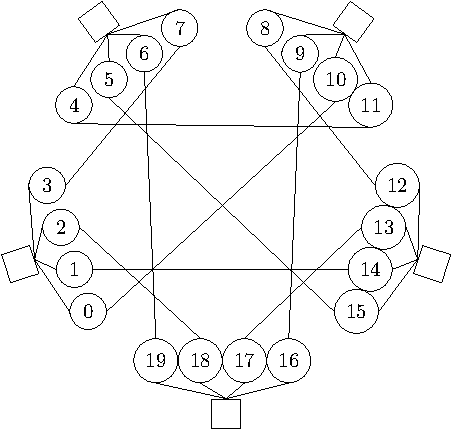
\includegraphics[width=1\textwidth]{figures/topologies/dcell-crop}
        \subcaption{Dcell$_1$ with 4 port switches \cite{GuoWTSZL08}}
    \end{minipage}\hfill
    \begin{minipage}{.53\textwidth}
        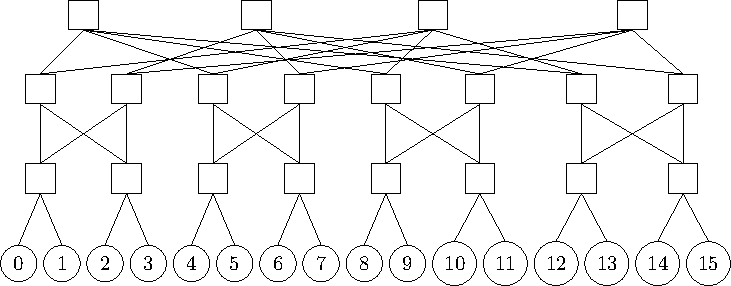
\includegraphics[width=\textwidth]{figures/topologies/fattree}
        \subcaption{Fat Tree with 4 port switches \cite{Al-FaresLV08}}

        \vspace{2.5em}

        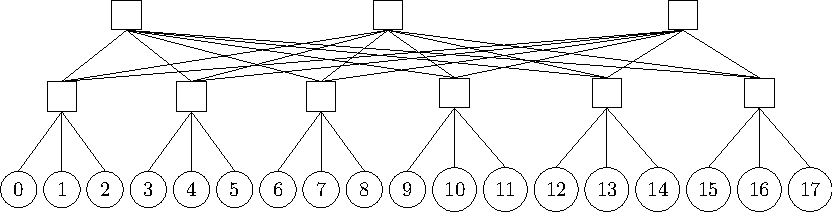
\includegraphics[width=\textwidth]{figures/topologies/leafspine}
        \subcaption{Leaf-Spine with 6 port switches \cite{Cisco19}}
    \end{minipage}\hfill
    \vspace{3em}
    \centering{
        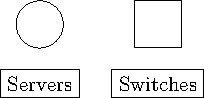
\includegraphics[width=0.2\textwidth]{figures/topologies/key}
    }
    \caption{Common datacenter topologies}
    \label{fig:topologies}
\end{figure*}

In this section, we describe the VNFPP and its constraints in detail. In the VNFPP, services must be placed on virtual machines in a datacenter so as to maximize multiple QoS objectives whilst minimizing energy consumption. The datacenter is a collection of servers interconnected by a network topology (see Fig. \ref{fig:topologies}). A service is a sequence of VNFs. Packets arrive at the first VNF in the service and must visit each VNF in sequence. A solution to the VNFPP places one or more instances of each VNF in the datacenter and specifies paths between VNFs to form services. 

The VNFPP has three objectives: two QoS metrics, latency and packet loss, and a cost metric, energy consumption. As service latency, packet loss and energy consumption conflict \cite{BillingsleyLMMG20} we formulate the VNFPP as a multi-objective optimization problem. Further, as services in a datacenter can number in the thousands it is not possible to treat each service quality metric as a separate objective. Instead, we aim to minimize the average service latency and the average service packet loss over all services, as well as the total energy consumption. Formally:

\begin{equation}
	\text{minimize} \ \textbf{F}\left(R_S\right) = \left(W, P, E\right)^T
	\label{eq:mo_formulation}
\end{equation}

\noindent where $R_S$ is the set of routes for each service, $W$ is the average service latency, $P$ is the average service packet loss and $E$ is the total electricity consumption of the datacenter. Several models exist to determine $W$, $P$ and $E$ for the VNFPP. This work uses the queueing theory model we proposed in \cite{BillingsleyLMMG19} and extended in \cite{BillingsleyJOURNAL}.

Finally, for a solution to the VNFPP to be feasible, it must satisfy two constraints. First, every VNF consumes some resources on a server. The total resources consumed by VNFs on a server cannot exceed the total resources of the server. Second, the solution must define one or more valid paths for each service. To be valid, a path must visit each VNF of the service in the order it appears in the service.
